\documentclass[10pt]{article}
\usepackage[a4paper,landscape,margin=8mm]{geometry}
\usepackage[T1]{fontenc}
\usepackage{tikz}
\usetikzlibrary{arrows.meta}
\usepackage[colorlinks=true,linkcolor=blue,urlcolor=blue]{hyperref}
\usepackage{parskip}
\usepackage{needspace}
\pagestyle{plain}
\begin{document}
\begin{center}
\phantomsection\label{map}{\Large Navier--Stokes: dependency map}

Arrows run from premise to consumer. Dashed GAP nodes remain unproved.
PAPER denotes a written argument; review scope appears on the following pages.

\resizebox{\textwidth}{!}{%
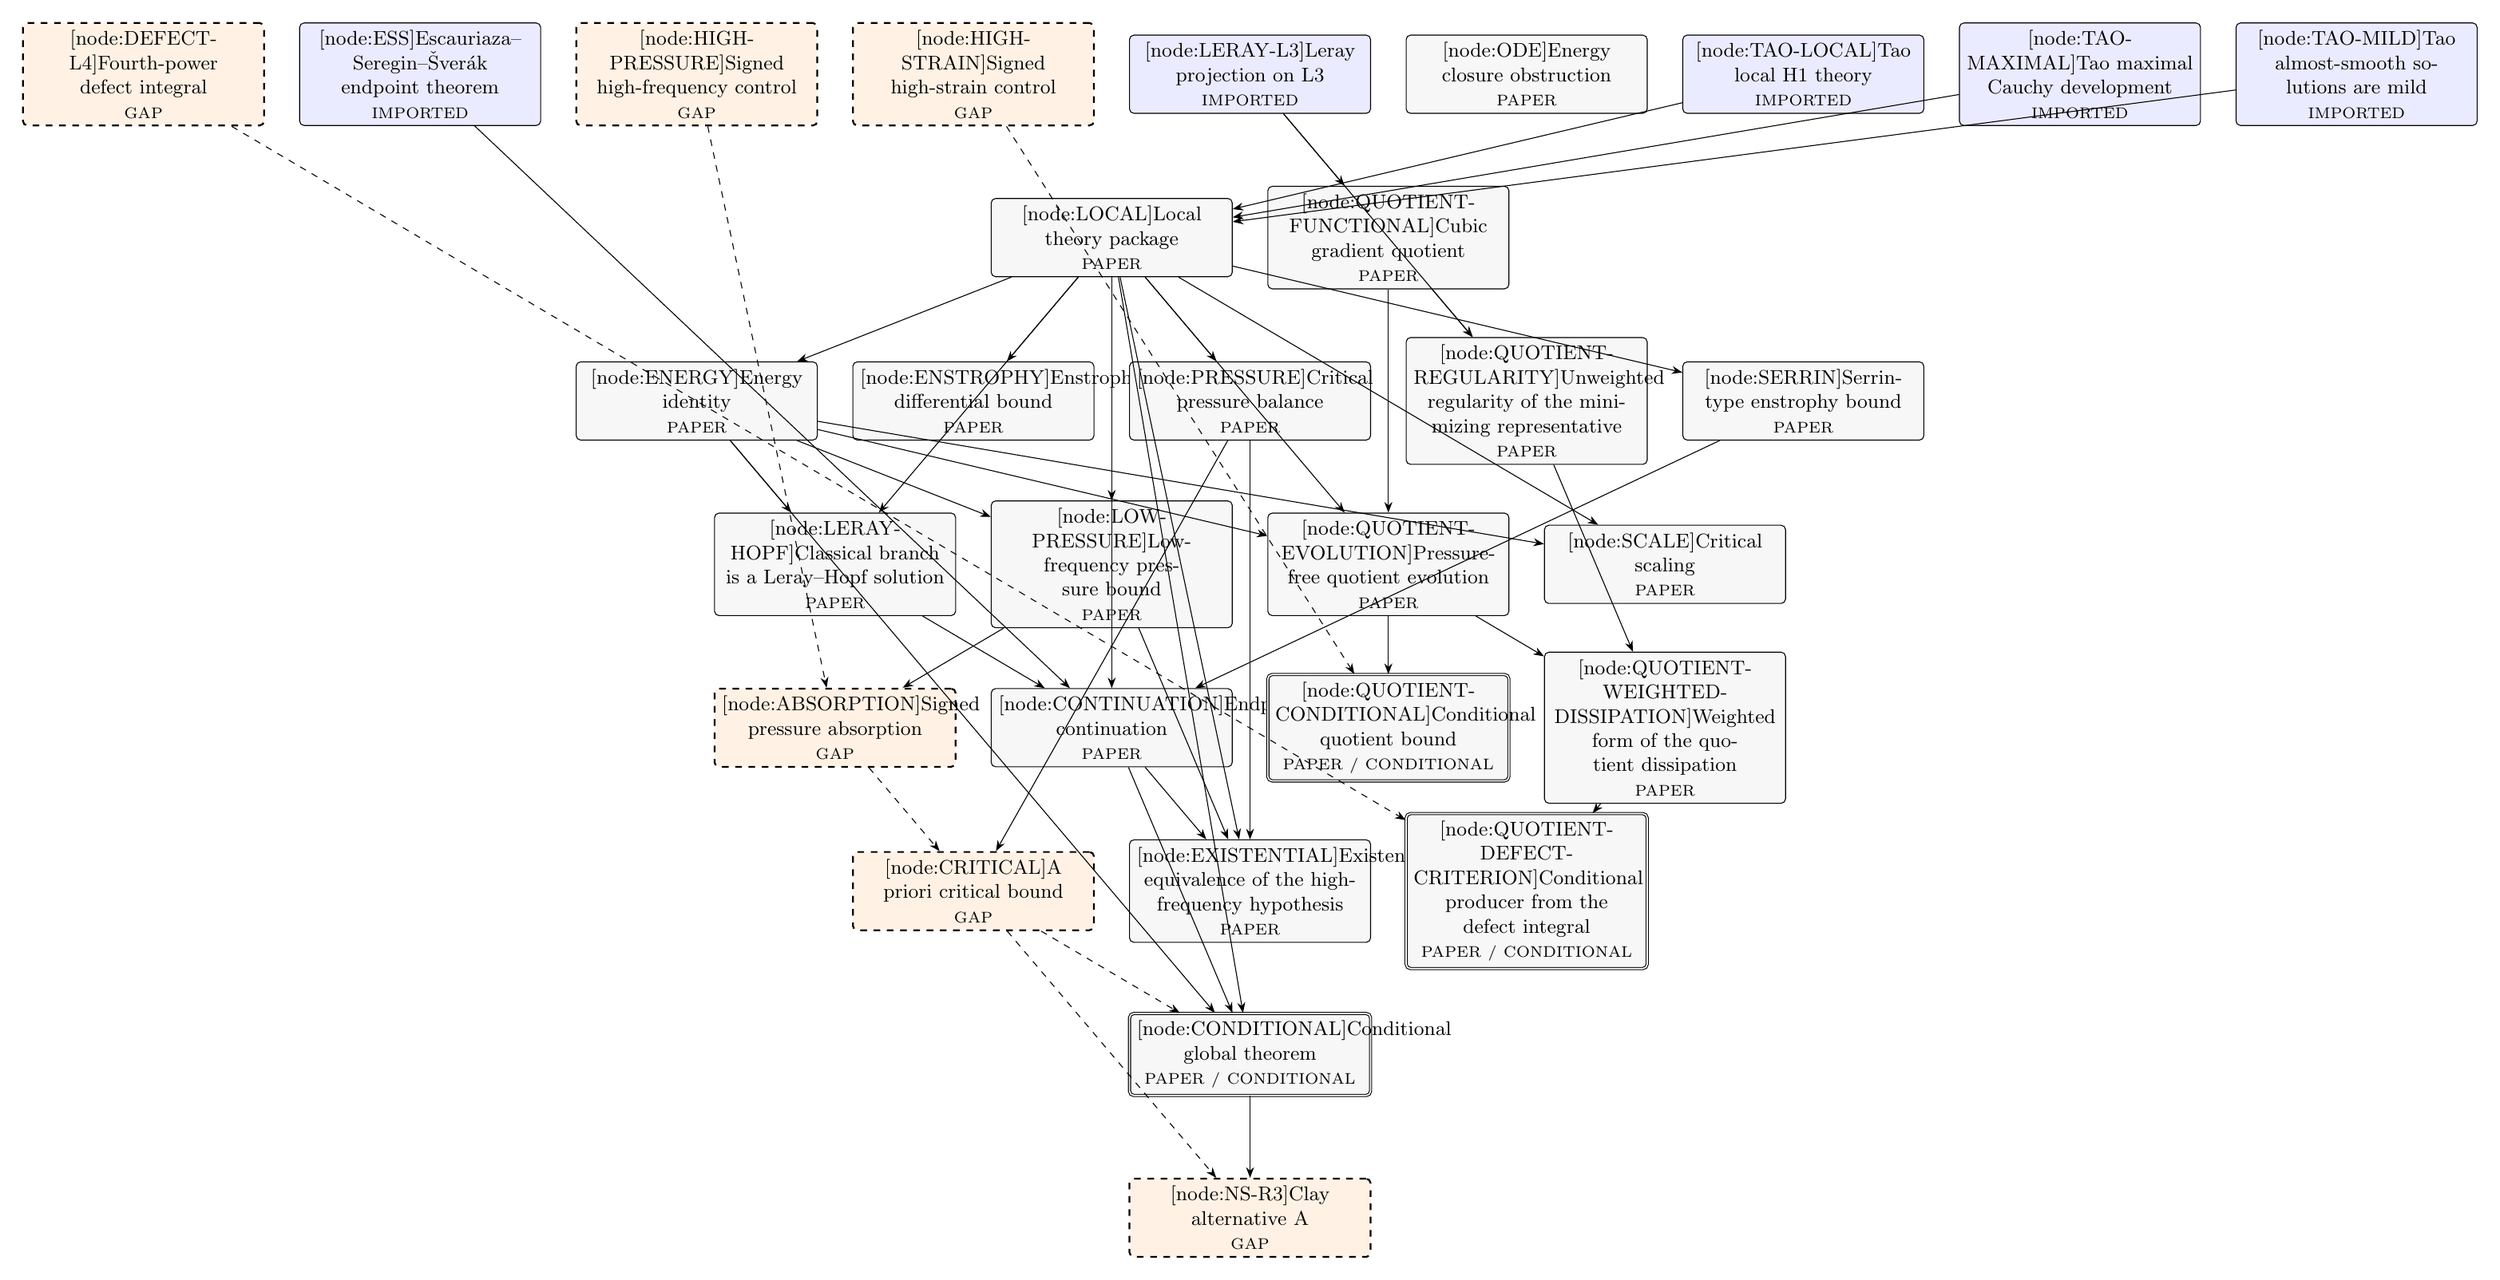
\begin{tikzpicture}[x=1cm,y=1cm,>=Stealth,
box/.style={draw,rounded corners=2pt,text width=3.6cm,minimum height=1.0cm,align=center,font=\small},
imported/.style={box,fill=blue!8},paper/.style={box,fill=black!3},
conditional/.style={box,fill=black!3,double},gap/.style={box,dashed,thick,fill=orange!10},
edge/.style={->,thin}]
\node[imported] (TAO-LOCAL) at (8.80,-0.00) {\hyperref[node:TAO-LOCAL]{Tao local H1 theory}\\{\scriptsize IMPORTED}};
\node[imported] (TAO-MAXIMAL) at (13.20,-0.00) {\hyperref[node:TAO-MAXIMAL]{Tao maximal Cauchy development}\\{\scriptsize IMPORTED}};
\node[imported] (TAO-MILD) at (17.60,-0.00) {\hyperref[node:TAO-MILD]{Tao almost-smooth solutions are mild}\\{\scriptsize IMPORTED}};
\node[paper] (LOCAL) at (-2.20,-2.60) {\hyperref[node:LOCAL]{Local theory package}\\{\scriptsize PAPER}};
\node[paper] (ENERGY) at (-8.80,-5.20) {\hyperref[node:ENERGY]{Energy identity}\\{\scriptsize PAPER}};
\node[paper] (SCALE) at (6.60,-7.80) {\hyperref[node:SCALE]{Critical scaling}\\{\scriptsize PAPER}};
\node[paper] (ENSTROPHY) at (-4.40,-5.20) {\hyperref[node:ENSTROPHY]{Enstrophy differential bound}\\{\scriptsize PAPER}};
\node[paper] (ODE) at (4.40,-0.00) {\hyperref[node:ODE]{Energy closure obstruction}\\{\scriptsize PAPER}};
\node[paper] (PRESSURE) at (0.00,-5.20) {\hyperref[node:PRESSURE]{Critical pressure balance}\\{\scriptsize PAPER}};
\node[paper] (LOW-PRESSURE) at (-2.20,-7.80) {\hyperref[node:LOW-PRESSURE]{Low-frequency pressure bound}\\{\scriptsize PAPER}};
\node[gap] (HIGH-PRESSURE) at (-8.80,-0.00) {\hyperref[node:HIGH-PRESSURE]{Signed high-frequency control}\\{\scriptsize GAP}};
\node[gap] (ABSORPTION) at (-6.60,-10.40) {\hyperref[node:ABSORPTION]{Signed pressure absorption}\\{\scriptsize GAP}};
\node[paper] (EXISTENTIAL) at (0.00,-13.00) {\hyperref[node:EXISTENTIAL]{Existential equivalence of the high-frequency hypothesis}\\{\scriptsize PAPER}};
\node[gap] (CRITICAL) at (-4.40,-13.00) {\hyperref[node:CRITICAL]{A priori critical bound}\\{\scriptsize GAP}};
\node[imported] (ESS) at (-13.20,-0.00) {\hyperref[node:ESS]{Escauriaza\textendash{}\allowbreak{}Seregin\textendash{}\allowbreak{}Šverák endpoint theorem}\\{\scriptsize IMPORTED}};
\node[paper] (LERAY-HOPF) at (-6.60,-7.80) {\hyperref[node:LERAY-HOPF]{Classical branch is a Leray\textendash{}\allowbreak{}Hopf solution}\\{\scriptsize PAPER}};
\node[paper] (SERRIN) at (8.80,-5.20) {\hyperref[node:SERRIN]{Serrin-type enstrophy bound}\\{\scriptsize PAPER}};
\node[paper] (CONTINUATION) at (-2.20,-10.40) {\hyperref[node:CONTINUATION]{Endpoint continuation}\\{\scriptsize PAPER}};
\node[conditional] (CONDITIONAL) at (0.00,-15.60) {\hyperref[node:CONDITIONAL]{Conditional global theorem}\\{\scriptsize PAPER / CONDITIONAL}};
\node[gap] (NS-R3) at (0.00,-18.20) {\hyperref[node:NS-R3]{Clay alternative A}\\{\scriptsize GAP}};
\node[imported] (LERAY-L3) at (0.00,-0.00) {\hyperref[node:LERAY-L3]{Leray projection on L3}\\{\scriptsize IMPORTED}};
\node[paper] (QUOTIENT-REGULARITY) at (4.40,-5.20) {\hyperref[node:QUOTIENT-REGULARITY]{Unweighted regularity of the minimizing representative}\\{\scriptsize PAPER}};
\node[paper] (QUOTIENT-FUNCTIONAL) at (2.20,-2.60) {\hyperref[node:QUOTIENT-FUNCTIONAL]{Cubic gradient quotient}\\{\scriptsize PAPER}};
\node[paper] (QUOTIENT-EVOLUTION) at (2.20,-7.80) {\hyperref[node:QUOTIENT-EVOLUTION]{Pressure-free quotient evolution}\\{\scriptsize PAPER}};
\node[gap] (HIGH-STRAIN) at (-4.40,-0.00) {\hyperref[node:HIGH-STRAIN]{Signed high-strain control}\\{\scriptsize GAP}};
\node[paper] (QUOTIENT-WEIGHTED-DISSIPATION) at (6.60,-10.40) {\hyperref[node:QUOTIENT-WEIGHTED-DISSIPATION]{Weighted form of the quotient dissipation}\\{\scriptsize PAPER}};
\node[gap] (DEFECT-L4) at (-17.60,-0.00) {\hyperref[node:DEFECT-L4]{Fourth-power defect integral}\\{\scriptsize GAP}};
\node[conditional] (QUOTIENT-DEFECT-CRITERION) at (4.40,-13.00) {\hyperref[node:QUOTIENT-DEFECT-CRITERION]{Conditional producer from the defect integral}\\{\scriptsize PAPER / CONDITIONAL}};
\node[conditional] (QUOTIENT-CONDITIONAL) at (2.20,-10.40) {\hyperref[node:QUOTIENT-CONDITIONAL]{Conditional quotient bound}\\{\scriptsize PAPER / CONDITIONAL}};
\draw[edge] (TAO-LOCAL) -- (LOCAL);
\draw[edge] (TAO-MAXIMAL) -- (LOCAL);
\draw[edge] (TAO-MILD) -- (LOCAL);
\draw[edge] (LOCAL) -- (ENERGY);
\draw[edge] (ENERGY) -- (SCALE);
\draw[edge] (LOCAL) -- (SCALE);
\draw[edge] (LOCAL) -- (ENSTROPHY);
\draw[edge] (LOCAL) -- (PRESSURE);
\draw[edge] (ENERGY) -- (LOW-PRESSURE);
\draw[edge] (LOCAL) -- (LOW-PRESSURE);
\draw[edge] (LOW-PRESSURE) -- (ABSORPTION);
\draw[edge,dashed] (HIGH-PRESSURE) -- (ABSORPTION);
\draw[edge] (LOW-PRESSURE) -- (EXISTENTIAL);
\draw[edge] (PRESSURE) -- (EXISTENTIAL);
\draw[edge] (CONTINUATION) -- (EXISTENTIAL);
\draw[edge] (LOCAL) -- (EXISTENTIAL);
\draw[edge] (PRESSURE) -- (CRITICAL);
\draw[edge,dashed] (ABSORPTION) -- (CRITICAL);
\draw[edge] (LOCAL) -- (LERAY-HOPF);
\draw[edge] (ENERGY) -- (LERAY-HOPF);
\draw[edge] (LOCAL) -- (SERRIN);
\draw[edge] (LOCAL) -- (CONTINUATION);
\draw[edge] (LERAY-HOPF) -- (CONTINUATION);
\draw[edge] (ESS) -- (CONTINUATION);
\draw[edge] (SERRIN) -- (CONTINUATION);
\draw[edge] (LOCAL) -- (CONDITIONAL);
\draw[edge] (ENERGY) -- (CONDITIONAL);
\draw[edge] (CONTINUATION) -- (CONDITIONAL);
\draw[edge,dashed] (CRITICAL) -- (CONDITIONAL);
\draw[edge] (CONDITIONAL) -- (NS-R3);
\draw[edge,dashed] (CRITICAL) -- (NS-R3);
\draw[edge] (LERAY-L3) -- (QUOTIENT-REGULARITY);
\draw[edge] (QUOTIENT-FUNCTIONAL) -- (QUOTIENT-REGULARITY);
\draw[edge] (LERAY-L3) -- (QUOTIENT-FUNCTIONAL);
\draw[edge] (LOCAL) -- (QUOTIENT-EVOLUTION);
\draw[edge] (ENERGY) -- (QUOTIENT-EVOLUTION);
\draw[edge] (QUOTIENT-FUNCTIONAL) -- (QUOTIENT-EVOLUTION);
\draw[edge] (QUOTIENT-REGULARITY) -- (QUOTIENT-WEIGHTED-DISSIPATION);
\draw[edge] (QUOTIENT-EVOLUTION) -- (QUOTIENT-WEIGHTED-DISSIPATION);
\draw[edge] (QUOTIENT-WEIGHTED-DISSIPATION) -- (QUOTIENT-DEFECT-CRITERION);
\draw[edge,dashed] (DEFECT-L4) -- (QUOTIENT-DEFECT-CRITERION);
\draw[edge] (QUOTIENT-EVOLUTION) -- (QUOTIENT-CONDITIONAL);
\draw[edge,dashed] (HIGH-STRAIN) -- (QUOTIENT-CONDITIONAL);
\end{tikzpicture}}

Phase I: reopened-2026-09-06-in-progress. Phase II: reopened-2026-09-06-target.
No terminal proof or counterexample is claimed.
\end{center}
\clearpage
\raggedright
Graph SHA-256: \texttt{377a3190407510641039a11a88d3ceb8}\texttt{54a6627367188a7533d7335f8ef3ec21}.
\Needspace{10\baselineskip}\section*{TAO-LOCAL: Tao local H1 theory}\phantomsection\label{node:TAO-LOCAL}
\textbf{Class:} IMPORTED. \textbf{Formal:} not started.

Tao 2013 Theorem 5.4 at unit viscosity on R3, verbatim, with its H1 data, H1 mild solution and normalised pressure definitions, including uniqueness of H1 mild solutions and smoothness for Schwartz data.

\textbf{Mechanism:} published local well-posedness theorem.

\textbf{Review:} Directly inspected at the published pages 52\textendash{}\allowbreak{}53; transcribed in cp02-local-theory.md and checked in cp02-review-local-theory-r2.md. Not a statement about maximal development or about viscosity other than one.

\textbf{Evidence:} \texttt{research/evidence/cp01-literature-statements.md}. Manuscript label: \texttt{thm:tao54}.

\textbf{Dependencies:} none. \hyperref[map]{Back to map}.

\Needspace{10\baselineskip}\section*{TAO-MAXIMAL: Tao maximal Cauchy development}\phantomsection\label{node:TAO-MAXIMAL}
\textbf{Class:} IMPORTED. \textbf{Formal:} not started.

Tao 2013 Corollary 5.8 at unit viscosity on R3, verbatim, with the incomplete mild H1 solution definition, giving for every finite horizon either a mild H1 solution or enstrophy blow-up before that horizon.

\textbf{Mechanism:} published dichotomy.

\textbf{Review:} Directly inspected at the published pages 56\textendash{}\allowbreak{}57; the passage from the per-horizon dichotomy to one maximal time is manuscript-owned (LOCAL).

\textbf{Evidence:} \texttt{research/evidence/cp01-literature-statements.md}. Manuscript label: \texttt{thm:tao58}.

\textbf{Dependencies:} none. \hyperref[map]{Back to map}.

\Needspace{10\baselineskip}\section*{TAO-MILD: Tao almost-smooth solutions are mild}\phantomsection\label{node:TAO-MILD}
\textbf{Class:} IMPORTED. \textbf{Formal:} not started.

Tao 2013 Corollary 4.3, verbatim, at unit viscosity on R3, showing that an almost smooth H1 solution becomes an H1 mild solution after pressure normalisation.

\textbf{Mechanism:} published pressure normalisation.

\textbf{Review:} Directly inspected at the published page 47 in cp02-local-theory.md; supplies the uniqueness class of classical solutions with arbitrary pressure.

\textbf{Evidence:} \texttt{research/evidence/cp01-literature-statements.md}. Manuscript label: \texttt{thm:tao43}.

\textbf{Dependencies:} none. \hyperref[map]{Back to map}.

\Needspace{10\baselineskip}\section*{LOCAL: Local theory package}\phantomsection\label{node:LOCAL}
\textbf{Class:} PAPER. \textbf{Formal:} not started.

For every viscosity and divergence-free Schwartz datum there is a maximal time Tstar in (0,infinity] and a classical branch, unique in the H1 mild class, such that on every compact interval of [0,Tstar) velocity and normalised pressure lie in C\textasciicircum{}j([0,T];H\textasciicircum{}k) for all j and k, are smooth with bounded derivatives, satisfy the equation pointwise with the given datum, and the enstrophy diverges as t tends to Tstar when Tstar is finite.

\textbf{Mechanism:} viscosity rescaling, gluing and supremum, Sobolev upgrade of the L-infinity-in-time bounds.

\textbf{Review:} Round-two audit cp02-review-local-theory-r2.md finds no invalid bridge; three scope wordings repaired at integration. Every other paper node cites this package.

\textbf{Evidence:} \texttt{research/evidence/cp02-local-theory.md}. Manuscript label: \texttt{prop:localtheory}.

\textbf{Dependencies:} \hyperref[node:TAO-LOCAL]{TAO-LOCAL}, \hyperref[node:TAO-MAXIMAL]{TAO-MAXIMAL}, \hyperref[node:TAO-MILD]{TAO-MILD}. \hyperref[map]{Back to map}.

\Needspace{10\baselineskip}\section*{ENERGY: Energy identity}\phantomsection\label{node:ENERGY}
\textbf{Class:} PAPER. \textbf{Formal:} not started.

On every compact classical interval, E(t) + 2 nu integral\_0\textasciicircum{}t Y(s) ds = E(0), where E is squared L2 velocity and Y is squared L2 gradient; hence the kinetic energy never exceeds its initial value and the enstrophy is time integrable up to Tstar.

\textbf{Mechanism:} divergence cancellation and integration by parts justified from the package.

\textbf{Review:} cp02-review-energy-enstrophy-r2.md PASS; every Fourier fact imported in one labelled lemma with an inspected source.

\textbf{Evidence:} \texttt{research/evidence/cp02-energy-enstrophy.md}. Manuscript label: \texttt{prop:energy}.

\textbf{Dependencies:} \hyperref[node:LOCAL]{LOCAL}. \hyperref[map]{Back to map}.

\Needspace{10\baselineskip}\section*{SCALE: Critical scaling}\phantomsection\label{node:SCALE}
\textbf{Class:} PAPER. \textbf{Formal:} not started.

The critical rescaling maps solutions to solutions with the same viscosity, preserves L3, scales squared L2 by lambda to the minus one, and the energy bounds yield L4 in time of L3 in space but not L-infinity in time of L3.

\textbf{Mechanism:} change of variables, Hoelder interpolation, Sobolev inequality on H1.

\textbf{Review:} cp02-review-energy-enstrophy-r2.md PASS; the norm half is machine-checked in navier-formal (eLpNorm\_dilate).

\textbf{Evidence:} \texttt{research/evidence/cp02-energy-enstrophy.md}. Manuscript label: \texttt{prop:scaling}.

\textbf{Dependencies:} \hyperref[node:ENERGY]{ENERGY}, \hyperref[node:LOCAL]{LOCAL}. \hyperref[map]{Back to map}.

\Needspace{10\baselineskip}\section*{ENSTROPHY: Enstrophy differential bound}\phantomsection\label{node:ENSTROPHY}
\textbf{Class:} PAPER. \textbf{Formal:} not started.

On a classical interval, one half Y prime plus nu over two times squared L2 Laplacian is at most C nu to the power minus three times Y cubed.

\textbf{Mechanism:} stretching identity, Gagliardo\textendash{}\allowbreak{}Nirenberg, Young.

\textbf{Review:} cp02-review-energy-enstrophy-r2.md PASS. Not used in the conditional chain.

\textbf{Evidence:} \texttt{research/evidence/cp02-energy-enstrophy.md}. Manuscript label: \texttt{prop:enstrophy}.

\textbf{Dependencies:} \hyperref[node:LOCAL]{LOCAL}. \hyperref[map]{Back to map}.

\Needspace{10\baselineskip}\section*{ODE: Energy closure obstruction}\phantomsection\label{node:ODE}
\textbf{Class:} PAPER. \textbf{Formal:} not started.

A positive scalar function can diverge at finite time while its time integral is finite and its derivative equals a constant times its cube.

\textbf{Mechanism:} explicit inverse-square-root example.

\textbf{Review:} Complete on the page; machine-checked in navier-formal (scalar\_obstruction\_exists). Not a Navier\textendash{}\allowbreak{}Stokes blowup solution.

\textbf{Evidence:} \texttt{research/evidence/cp02-energy-enstrophy.md}. Manuscript label: \texttt{prop:ode}.

\textbf{Dependencies:} none. \hyperref[map]{Back to map}.

\Needspace{10\baselineskip}\section*{PRESSURE: Critical pressure balance}\phantomsection\label{node:PRESSURE}
\textbf{Class:} PAPER. \textbf{Formal:} not started.

In integrated form on every compact classical interval, one third of the cubed L3 norm at time t minus at time s plus nu times the integrated weighted cubic dissipation D3 equals the integrated signed pressure work P3, with D3 and P3 defined through the transpose gradient applied to the velocity and vanishing integrands on the zero set.

\textbf{Mechanism:} regularised speed, spatial cutoff, two limits with displayed error terms.

\textbf{Review:} cp02-review-pressure-r2.md finds no invalid bridge; the duplicate pressure-convention lemma is removed at integration in favour of the local-theory lemma. Differential form is a remark, not a claim.

\textbf{Evidence:} \texttt{research/evidence/cp02-pressure.md}. Manuscript label: \texttt{prop:pressure}.

\textbf{Dependencies:} \hyperref[node:LOCAL]{LOCAL}. \hyperref[map]{Back to map}.

\Needspace{10\baselineskip}\section*{LOW-PRESSURE: Low-frequency pressure bound}\phantomsection\label{node:LOW-PRESSURE}
\textbf{Class:} PAPER. \textbf{Formal:} not started.

For the fixed inhomogeneous low-pass profile and every integer J, horizon H and tau below min(H,Tstar), the accumulated low-frequency pressure work is bounded by an explicit constant times 2\textasciicircum{}(3J) times the fourth power of the initial L2 norm times the square root of H/(2 nu).

\textbf{Mechanism:} L1 frequency bound of the low-pass Riesz multiplier and Cauchy\textendash{}\allowbreak{}Schwarz in time.

\textbf{Review:} cp02-review-lowpressure.md PASS with two one-line insertions applied at integration; explicit constant path recorded.

\textbf{Evidence:} \texttt{research/evidence/cp02-lowpressure.md}. Manuscript label: \texttt{prop:lowpressure}.

\textbf{Dependencies:} \hyperref[node:ENERGY]{ENERGY}, \hyperref[node:LOCAL]{LOCAL}. \hyperref[map]{Back to map}.

\Needspace{10\baselineskip}\section*{HIGH-PRESSURE: Signed high-frequency control}\phantomsection\label{node:HIGH-PRESSURE}
\textbf{Class:} GAP. \textbf{Formal:} not started.

There exists a fixed theta in [0,1) such that for every datum, viscosity and positive finite horizon H there exist an integer cutoff J and a finite nonnegative remainder making accumulated high-frequency pressure work at most theta nu times accumulated cubic dissipation plus that remainder, for every tau less than min(H,Tstar).

\textbf{Mechanism:} new signed time-integrated pressure estimate on actual trajectories.

\textbf{Review:} Open. At these quantifiers equivalent to global continuation of the strong branch (prop:existential-equivalence). The HF02\textendash{}\allowbreak{}HF16 obstructions constrain specific mechanisms; HF17\textendash{}\allowbreak{}HF18 supply the alternative quotient route with an audited coercive dissipation identity. No arbitrary-data producer is proved.

\textbf{Evidence:} \texttt{research/evidence/frequency.md}. Manuscript label: \texttt{hyp:highpressure}.

\textbf{Dependencies:} none. \hyperref[map]{Back to map}.

\Needspace{10\baselineskip}\section*{ABSORPTION: Signed pressure absorption}\phantomsection\label{node:ABSORPTION}
\textbf{Class:} GAP. \textbf{Formal:} not started.

There exists a fixed theta in [0,1) such that for every datum, viscosity and finite horizon H there is a finite a priori A with integrated signed pressure work up to every tau less than min(H,Tstar) at most theta nu times integrated cubic dissipation plus A.

\textbf{Mechanism:} split pressure work into the proved low-frequency bound and the unproved high-frequency estimate.

\textbf{Review:} Open. Follows from LOW-PRESSURE and HIGH-PRESSURE with A the sum of the two remainders (lem:absorption-split).

\textbf{Evidence:} \texttt{research/evidence/architecture.md}. Manuscript label: \texttt{hyp:absorption}.

\textbf{Dependencies:} \hyperref[node:LOW-PRESSURE]{LOW-PRESSURE}, \hyperref[node:HIGH-PRESSURE]{HIGH-PRESSURE}. \hyperref[map]{Back to map}.

\Needspace{10\baselineskip}\section*{EXISTENTIAL: Existential equivalence of the high-frequency hypothesis}\phantomsection\label{node:EXISTENTIAL}
\textbf{Class:} PAPER. \textbf{Formal:} not started.

At its stated quantifiers, the high-frequency hypothesis holds if and only if every Schwartz-data classical branch is global; the forward direction runs through the conditional chain and the converse uses the local theory package on the global branch with cutoff zero and theta zero.

\textbf{Mechanism:} chain of implications and an explicit witness on a global branch.

\textbf{Review:} cp02-review-lowpressure.md PASS. This is a logical equivalence, not a method for proving either side.

\textbf{Evidence:} \texttt{research/evidence/cp02-lowpressure.md}. Manuscript label: \texttt{prop:existential-equivalence}.

\textbf{Dependencies:} \hyperref[node:LOW-PRESSURE]{LOW-PRESSURE}, \hyperref[node:PRESSURE]{PRESSURE}, \hyperref[node:CONTINUATION]{CONTINUATION}, \hyperref[node:LOCAL]{LOCAL}. \hyperref[map]{Back to map}.

\Needspace{10\baselineskip}\section*{CRITICAL: A priori critical bound}\phantomsection\label{node:CRITICAL}
\textbf{Class:} GAP. \textbf{Formal:} not started.

For each viscosity, Schwartz datum, and finite horizon H, there exists a finite M depending only on these inputs such that the classical branch obeys sup over 0 < t < min(H,Tstar) of its L3 norm at most M.

\textbf{Mechanism:} integrate the pressure balance under the unproved absorption estimate.

\textbf{Review:} Open. Implied by ABSORPTION with M cubed equal to the initial cubed L3 norm plus 3A (cor:absorption-consequence); alternatively by the quotient route under HIGH-STRAIN (prop:quotient-conditional).

\textbf{Evidence:} \texttt{research/evidence/architecture.md}. Manuscript label: \texttt{hyp:critical}.

\textbf{Dependencies:} \hyperref[node:PRESSURE]{PRESSURE}, \hyperref[node:ABSORPTION]{ABSORPTION}. \hyperref[map]{Back to map}.

\Needspace{10\baselineskip}\section*{ESS: Escauriaza\textendash{}\allowbreak{}Seregin\textendash{}\allowbreak{}Šverák endpoint theorem}\phantomsection\label{node:ESS}
\textbf{Class:} IMPORTED. \textbf{Formal:} not started.

ESS 2003 Theorem 1.3, verbatim, at unit viscosity on R3, with the Leray\textendash{}\allowbreak{}Hopf weak solution conditions (1.3)\textendash{}\allowbreak{}(1.7) and the mixed-norm convention, so that a Leray\textendash{}\allowbreak{}Hopf weak solution on Q\_T that lies in L-infinity in time of L3 in space belongs to L5 of Q\_T and is smooth and unique on Q\_T.

\textbf{Mechanism:} published backward-uniqueness theorem.

\textbf{Review:} Directly inspected at the published pages 211\textendash{}\allowbreak{}214 in cp02-continuation.md; the L3 in the theorem is the space norm and L\_\{3,infinity\} means L-infinity in time. GKP Theorem 4 is corroboration only.

\textbf{Evidence:} \texttt{research/evidence/cp01-literature-statements.md}. Manuscript label: \texttt{thm:ess}.

\textbf{Dependencies:} none. \hyperref[map]{Back to map}.

\Needspace{10\baselineskip}\section*{LERAY-HOPF: Classical branch is a Leray\textendash{}\allowbreak{}Hopf solution}\phantomsection\label{node:LERAY-HOPF}
\textbf{Class:} PAPER. \textbf{Formal:} not started.

The unit-viscosity rescaling of the classical branch is a Leray\textendash{}\allowbreak{}Hopf weak solution on every Q\_T with T at most the rescaled maximal time, in the exact sense of ESS conditions (1.3)\textendash{}\allowbreak{}(1.7), with bounds uniform up to the maximal time.

\textbf{Mechanism:} density of smooth compactly supported solenoidal fields, weak continuity, energy identity, weak limit at the endpoint.

\textbf{Review:} cp02-review-continuation-r2.md PASS; the solenoidal density lemma is proved in full via Biot\textendash{}\allowbreak{}Savart, Hardy and mollification.

\textbf{Evidence:} \texttt{research/evidence/cp02-continuation.md}. Manuscript label: \texttt{lem:leray-hopf}.

\textbf{Dependencies:} \hyperref[node:LOCAL]{LOCAL}, \hyperref[node:ENERGY]{ENERGY}. \hyperref[map]{Back to map}.

\Needspace{10\baselineskip}\section*{SERRIN: Serrin-type enstrophy bound}\phantomsection\label{node:SERRIN}
\textbf{Class:} PAPER. \textbf{Formal:} not started.

If the classical branch lies in L5 of space-time up to T, then its enstrophy stays bounded up to T by the initial enstrophy times an exponential of an explicit constant times nu to the minus four times the integrated fifth power of the L5 norm.

\textbf{Mechanism:} enstrophy identity, Hoelder, interpolation, Sobolev, Plancherel, Young, Gronwall.

\textbf{Review:} cp02-review-continuation-r2.md PASS with every exponent recomputed.

\textbf{Evidence:} \texttt{research/evidence/cp02-continuation.md}. Manuscript label: \texttt{lem:serrin-enstrophy}.

\textbf{Dependencies:} \hyperref[node:LOCAL]{LOCAL}. \hyperref[map]{Back to map}.

\Needspace{10\baselineskip}\section*{CONTINUATION: Endpoint continuation}\phantomsection\label{node:CONTINUATION}
\textbf{Class:} PAPER. \textbf{Formal:} not started.

If the maximal time of the Schwartz-data classical branch is finite then the supremum of its L3 norm over [0,Tstar) is infinite; equivalently a finite uniform L3 bound forces a global branch.

\textbf{Mechanism:} viscosity normalisation, ESS gives L5, the Serrin-type bound contradicts the blow-up alternative.

\textbf{Review:} cp02-review-continuation-r2.md PASS. No L3 uniqueness theorem is imported; the identification step of the earlier manuscript is gone.

\textbf{Evidence:} \texttt{research/evidence/cp02-continuation.md}. Manuscript label: \texttt{thm:continuation}.

\textbf{Dependencies:} \hyperref[node:LOCAL]{LOCAL}, \hyperref[node:LERAY-HOPF]{LERAY-HOPF}, \hyperref[node:ESS]{ESS}, \hyperref[node:SERRIN]{SERRIN}. \hyperref[map]{Back to map}.

\Needspace{10\baselineskip}\section*{CONDITIONAL: Conditional global theorem}\phantomsection\label{node:CONDITIONAL}
\textbf{Class:} PAPER / CONDITIONAL. \textbf{Formal:} not started.

Assuming the critical bound for every admissible input, every Schwartz datum and viscosity give a global classical branch, smooth with the normalised pressure on R3 times the closed half-line, with kinetic energy never exceeding its initial value; this is Clay alternative A.

\textbf{Mechanism:} contradiction at a finite maximal time, then the package on every compact interval.

\textbf{Review:} cp02-review-continuation-r2.md PASS; Fefferman's clauses checked one by one. CRITICAL remains unproved.

\textbf{Evidence:} \texttt{research/evidence/cp02-continuation.md}. Manuscript label: \texttt{thm:conditional}.

\textbf{Dependencies:} \hyperref[node:LOCAL]{LOCAL}, \hyperref[node:ENERGY]{ENERGY}, \hyperref[node:CONTINUATION]{CONTINUATION}, \hyperref[node:CRITICAL]{CRITICAL}. \hyperref[map]{Back to map}.

\Needspace{10\baselineskip}\section*{NS-R3: Clay alternative A}\phantomsection\label{node:NS-R3}
\textbf{Class:} GAP. \textbf{Formal:} not started.

Every smooth divergence-free rapidly decreasing initial velocity on R3 has a global smooth unforced Navier\textendash{}\allowbreak{}Stokes velocity and pressure of uniformly bounded kinetic energy, for every positive viscosity.

\textbf{Mechanism:} discharge the critical estimate in the conditional theorem.

\textbf{Review:} Open. No complete proof or counterexample.

\textbf{Evidence:} \texttt{docs/proof.md}. Manuscript label: \texttt{def:target}.

\textbf{Dependencies:} \hyperref[node:CONDITIONAL]{CONDITIONAL}, \hyperref[node:CRITICAL]{CRITICAL}. \hyperref[map]{Back to map}.

\Needspace{10\baselineskip}\section*{LERAY-L3: Leray projection on L3}\phantomsection\label{node:LERAY-L3}
\textbf{Class:} IMPORTED. \textbf{Formal:} not started.

The Leray projection extends from L2 to a bounded operator on L3 of R3 that annihilates gradients; Calderón\textendash{}\allowbreak{}Zygmund boundedness of the Riesz transforms.

\textbf{Mechanism:} Calderón\textendash{}\allowbreak{}Zygmund theory.

\textbf{Review:} Stated in Tao 2013 page 38 (directly inspected) with Stein as the underlying source (metadata). Phase II must prove it from Mathlib; it is textbook, not a research theorem.

\textbf{Evidence:} \texttt{research/evidence/cp01-literature-statements.md}. Manuscript label: \texttt{lem:leray}.

\textbf{Dependencies:} none. \hyperref[map]{Back to map}.

\Needspace{10\baselineskip}\section*{QUOTIENT-REGULARITY: Unweighted regularity of the minimizing representative}\phantomsection\label{node:QUOTIENT-REGULARITY}
\textbf{Class:} PAPER. \textbf{Formal:} not started.

For every solenoidal H1 field on R3 the cubic minimizing representative has weak derivatives in L2, with squared gradient at most five quarters of the datum's and squared divergence at most one quarter, with no smallness; the divergence defect lies in L2 and equals the radial speed derivative almost everywhere including across the zero set, the vorticity vanishes almost everywhere on that zero set, and the mixed-pressure pairing holds with no hypothesis on the defect.

\textbf{Mechanism:} regularized minimization, a matrix inequality conditioned on the Euler-Lagrange relation, and the two Fourier div-curl identities.

\textbf{Review:} Audited PASS in hf23-review-regularity-core.md with three expository repairs applied at import; nine independent refutation attempts failed, including spectral minimisations on data whose minimizer vanishes. Discharges the weak-derivative hypothesis the earlier evidence carried, so every item gated on it is unconditional; the remaining hypothesis of that pair, the defect in L three halves, is bypassed rather than proved. Bounds no time integral of the squared enstrophy, so the open producer is untouched.

\textbf{Evidence:} \texttt{research/evidence/hf23-divcurl-continuation.md}. Manuscript label: \texttt{prop:quotient-divcurl}.

\textbf{Dependencies:} \hyperref[node:LERAY-L3]{LERAY-L3}, \hyperref[node:QUOTIENT-FUNCTIONAL]{QUOTIENT-FUNCTIONAL}. \hyperref[map]{Back to map}.

\Needspace{10\baselineskip}\section*{QUOTIENT-FUNCTIONAL: Cubic gradient quotient}\phantomsection\label{node:QUOTIENT-FUNCTIONAL}
\textbf{Class:} PAPER. \textbf{Formal:} not started.

The cubic L3 distance to the closed gradient subspace has a unique minimising representative w with divergence-free |w|w, is comparable to the cubed L3 norm on solenoidal fields, is cubic homogeneous and invariant under the critical scaling, is nonincreasing under heat, and is Fréchet differentiable with derivative the pairing against |w|w, which annihilates gradients.

\textbf{Mechanism:} reflexivity and strict convexity of L3, Leray projection, Gaussian convolution, uniform monotonicity of the cubic map.

\textbf{Review:} cp02-review-quotient-functional.md PASS. Related work is nonlinear Hodge theory and Kato's L\textasciicircum{}p Lyapunov functions; no novelty claim.

\textbf{Evidence:} \texttt{research/evidence/cp02-quotient-functional.md}. Manuscript label: \texttt{prop:quotient-derivative}.

\textbf{Dependencies:} \hyperref[node:LERAY-L3]{LERAY-L3}. \hyperref[map]{Back to map}.

\Needspace{10\baselineskip}\section*{QUOTIENT-EVOLUTION: Pressure-free quotient evolution}\phantomsection\label{node:QUOTIENT-EVOLUTION}
\textbf{Class:} PAPER. \textbf{Formal:} not started.

Along the classical branch on every compact interval, the quotient functional is absolutely continuous with derivative minus nu times a nonnegative dissipation minus the transport pairing of the gradient part against the strain, the pressure gradient being annihilated; the low-strain part is bounded by an input coefficient times the functional.

\textbf{Mechanism:} chain rule along a C1 curve in L3, heat generator sign, inner variation by the volume-preserving flow, Bernstein.

\textbf{Review:} cp02-review-quotient-evolution-r2.md PASS; Liouville's formula and the flow lemma are proved in full. HF18 identifies the dissipation with the coercive weighted cubic dissipation of the representative.

\textbf{Evidence:} \texttt{research/evidence/cp02-quotient-evolution.md}. Manuscript label: \texttt{prop:quotient-evolution}.

\textbf{Dependencies:} \hyperref[node:LOCAL]{LOCAL}, \hyperref[node:ENERGY]{ENERGY}, \hyperref[node:QUOTIENT-FUNCTIONAL]{QUOTIENT-FUNCTIONAL}. \hyperref[map]{Back to map}.

\Needspace{10\baselineskip}\section*{HIGH-STRAIN: Signed high-strain control}\phantomsection\label{node:HIGH-STRAIN}
\textbf{Class:} GAP. \textbf{Formal:} not started.

For every datum, viscosity, horizon and input-selected cutoff there is a finite input-only remainder such that the accumulated high-strain transport pairing is at most theta nu times the accumulated quotient dissipation plus that remainder, uniformly below min(H,Tstar), with theta at most one.

\textbf{Mechanism:} new signed time-integrated strain estimate on actual trajectories.

\textbf{Review:} Open. The audited HF18 bound |K| <= C Q\textasciicircum{}(1/3) D\_3(w) closes only under critical smallness. The audited HF20 sign test (hf20-review-harmonic-strain-test.md) excludes two further mechanism classes, namely universal monotonicity of the quotient and instantaneous absorption of the full transport term with an energy-only remainder; it leaves this spacetime hypothesis untouched, since that concerns the high-strain part with a datum-dependent remainder. Recorded in the manuscript as rem:no-monotone, whose second paragraph now excludes a fixed-cutoff energy-only remainder on genuine trajectories for every fixed cutoff, strengthening the earlier instantaneous exclusion to a time-integrated one. The audited HF23 regularity result (QUOTIENT-REGULARITY) discharges the weak-derivative hypothesis this route carried, but bounds no time integral of the squared enstrophy and so leaves this hypothesis untouched. The audited HF21 crossing lane (hf21-review-crossing-sign-structure.md) further normalises this hypothesis; by rem:highstrain-normalisation the Gronwall term and the frequency split are removable up to an input-only change of remainder, and by the added sentence of rem:highstrain-scope signed pressure absorption implies this hypothesis with an explicit remainder, so the two open routes are ordered rather than independent. The audited HF25 criterion adds a second ordered alternative, DEFECT-L4, which implies this hypothesis at theta equal to zero through QUOTIENT-DEFECT-CRITERION but is itself implied by classical gradient criteria on the same line, so this one-way comparison alone proves no strict improvement; the pending quotient-clock supplement supplies a reverse finiteness implication on actual branches. Alternative producer of CRITICAL, not an additional required lemma.

\textbf{Evidence:} \texttt{research/evidence/hf18-hodge-regularity.md}. Manuscript label: \texttt{hyp:highstrain}.

\textbf{Dependencies:} none. \hyperref[map]{Back to map}.

\Needspace{10\baselineskip}\section*{QUOTIENT-WEIGHTED-DISSIPATION: Weighted form of the quotient dissipation}\phantomsection\label{node:QUOTIENT-WEIGHTED-DISSIPATION}
\textbf{Class:} PAPER. \textbf{Formal:} not started.

Along the classical branch the quotient dissipation equals the weighted Dirichlet integral of the minimizing representative, the field |w|\textasciicircum{}(1/2)w lies in H1, the dissipation is at least eight ninths of that field's squared gradient, and the cube of the representative's L9 norm is bounded by a Sobolev multiple of the dissipation.

\textbf{Mechanism:} chain rule for the cubic duality map, a two-sided pointwise comparison affine in the angle cosine, and generalised dominated convergence of the difference quotients.

\textbf{Review:} Audited PASS WITH SCOPE in hf25-review-defect-criterion.md and imported with the prescribed repairs. Uses no uniform convexity and no Clarkson input. Asserts nothing in either direction about comparison with D3; the lower bound is on the representative, not on the datum.

\textbf{Evidence:} \texttt{research/evidence/hf25-beyond-hf21-continuation.md}. Manuscript label: \texttt{lem:qe-weighted-dissipation}.

\textbf{Dependencies:} \hyperref[node:QUOTIENT-REGULARITY]{QUOTIENT-REGULARITY}, \hyperref[node:QUOTIENT-EVOLUTION]{QUOTIENT-EVOLUTION}. \hyperref[map]{Back to map}.

\Needspace{10\baselineskip}\section*{DEFECT-L4: Fourth-power defect integral}\phantomsection\label{node:DEFECT-L4}
\textbf{Class:} GAP. \textbf{Formal:} not started.

For every datum, viscosity and horizon there is a finite input-only bound for the time integral of the fourth power of the L2 norm of the divergence defect of the minimizing representative, uniformly below min(H,Tstar).

\textbf{Mechanism:} new time-integrability estimate for the divergence of the representative.

\textbf{Review:} Open. The pointwise bound ||sigma||\_2 <= (1/2)||grad u||\_2 implies the defect condition from the classical gradient condition, not the opposite by itself; earlier not-weaker wording reversed that implication. The independently unaudited QUOTIENT-DISSIPATION-CLOCK supplement now proves a quantitative reverse finiteness implication on actual selected branches, excluding the previously undecided separation. This is a pending component proof, not a node promotion or a strict improvement over classical trajectory criteria. The energy budget still supplies only the square time integral; no arbitrary-data fourth-power producer is proved.

\textbf{Evidence:} \texttt{research/evidence/hf25-beyond-hf21-continuation.md}. Manuscript label: \texttt{eq:qe-defect-hypothesis}.

\textbf{Dependencies:} none. \hyperref[map]{Back to map}.

\Needspace{10\baselineskip}\section*{QUOTIENT-DEFECT-CRITERION: Conditional producer from the defect integral}\phantomsection\label{node:QUOTIENT-DEFECT-CRITERION}
\textbf{Class:} PAPER / CONDITIONAL. \textbf{Formal:} not started.

Under the fourth-power defect hypothesis the quotient obeys a Gronwall inequality with exponent the defect integral, bounding the quotient, the accumulated dissipation and the target product by explicit input-only constants, hence supplying the high-strain hypothesis at theta equal to zero.

\textbf{Mechanism:} an L2 pairing entry for the mixed pressure, interpolation between the cubic and ninth-power norms, exact Young maximisation, and Gronwall.

\textbf{Review:} Audited PASS WITH SCOPE in hf25-review-defect-criterion.md and imported with the mandatory scope remark rem:qe-defect-scope. Conditional consumer; DEFECT-L4 is unproved. No strict improvement over classical trajectory criteria is claimed; see the pending quantitative quotient-clock supplement. No progress toward a proof is claimed by this node's presence.

\textbf{Evidence:} \texttt{research/evidence/hf25-beyond-hf21-continuation.md}. Manuscript label: \texttt{cor:qe-defect-producer}.

\textbf{Dependencies:} \hyperref[node:QUOTIENT-WEIGHTED-DISSIPATION]{QUOTIENT-WEIGHTED-DISSIPATION}, \hyperref[node:DEFECT-L4]{DEFECT-L4}. \hyperref[map]{Back to map}.

\Needspace{10\baselineskip}\section*{QUOTIENT-CONDITIONAL: Conditional quotient bound}\phantomsection\label{node:QUOTIENT-CONDITIONAL}
\textbf{Class:} PAPER / CONDITIONAL. \textbf{Formal:} not started.

Under the high-strain hypothesis, Gronwall bounds the quotient functional, hence the L3 norm, on every finite horizon by an input-only constant; this supplies the critical bound by the quotient route.

\textbf{Mechanism:} integration and Gronwall.

\textbf{Review:} cp02-review-quotient-evolution-r2.md PASS. Conditional consumer; HIGH-STRAIN is unproved.

\textbf{Evidence:} \texttt{research/evidence/cp02-quotient-evolution.md}. Manuscript label: \texttt{prop:quotient-conditional}.

\textbf{Dependencies:} \hyperref[node:QUOTIENT-EVOLUTION]{QUOTIENT-EVOLUTION}, \hyperref[node:HIGH-STRAIN]{HIGH-STRAIN}. \hyperref[map]{Back to map}.

\clearpage\section*{Review-pending component: Direct nonendpoint dissipation-clock continuation}
\textbf{Not a promoted claim or an arbitrary-data producer.}

author-checked-independent-audit-pending. Full component derivations only; no arbitrary-data producer and no graph-node promotion.

\textbf{Evidence:} \texttt{research/evidence/2026-09-06-dissipation-clock.md}.

\textbf{Manuscript labels:} \texttt{dc:l9}, \texttt{dc:clock}, \texttt{dc:strict}, \texttt{dc:barrier}, \texttt{dc:nonlinear}, \texttt{dc:scalar}.
\clearpage\section*{Review-pending component: Near-2 unweighted defect regularity}
\textbf{Not a promoted claim or an arbitrary-data producer.}

author-checked-independent-audit-pending. A uniform spatial exponent interval with an additional gradient integrability hypothesis; not an all-exponent weighted estimate or a temporal producer.

\textbf{Evidence:} \texttt{research/evidence/2026-09-06-defect-extensions.md}.

\textbf{Manuscript labels:} \texttt{de:fixedpoint}, \texttt{de:near2}.
\clearpage\section*{Review-pending component: Quotient clock and no finiteness separation}
\textbf{Not a promoted claim or an arbitrary-data producer.}

author-checked-independent-audit-pending. Quantitative defect-enstrophy finiteness equivalence on actual branches; no arbitrary-data fourth-power estimate and no node promotion.

\textbf{Evidence:} \texttt{research/evidence/2026-09-06-defect-extensions.md}.

\textbf{Manuscript labels:} \texttt{de:quotient-clock}, \texttt{de:no-separation}.
\clearpage\section*{Review-pending component: Conformal moment and spatial defect bounds}
\textbf{Not a promoted claim or an arbitrary-data producer.}

author-checked-independent-audit-pending. Finite-energy representative and L3/2 defect under a weighted-gradient hypothesis, proved at every classical time with input-only integrated moment budgets for Schwartz data; supercritical time control only, no arbitrary-data critical producer or node promotion.

\textbf{Evidence:} \texttt{research/evidence/2026-09-06-conformal-moment.md}.

\textbf{Manuscript labels:} \texttt{cm:covariance}, \texttt{cm:inverted-h1}, \texttt{cm:snapshot}, \texttt{cm:moment}, \texttt{cm:spacetime}, \texttt{cm:scaling-test}.
\clearpage\section*{Review-pending component: Signed defect and one-sided form clock}
\textbf{Not a promoted claim or an arbitrary-data producer.}

author-checked-independent-audit-pending. Exact signed cancellation, smaller fourth-power coefficient and an explicit conditional defect bound from a critical one-sided form clock; independent audit pending, no arbitrary-data clock bound or graph-node promotion.

\textbf{Evidence:} \texttt{research/evidence/2026-09-06-signed-defect.md}.

\textbf{Manuscript labels:} \texttt{sd:cancellation}, \texttt{sd:improved}, \texttt{sd:form-clock}, \texttt{sd:missing-bound-consumer}, \texttt{sd:tail}.
\clearpage\section*{Review-pending component: Speed-shell cancellation and effective defect}
\textbf{Not a promoted claim or an arbitrary-data producer.}

author-checked-independent-audit-pending. Exact shell cancellation, speed-only projection residual, measurable depleted defect and null-corrected form bounds; pending signed-work and quotient-clock dependencies explicit, no arbitrary-data temporal producer or node promotion.

\textbf{Evidence:} \texttt{research/evidence/2026-09-06-speed-shell.md}.

\textbf{Manuscript labels:} \texttt{ss:shell}, \texttt{ss:residual}, \texttt{ss:clock}, \texttt{ss:gauge}, \texttt{ss:consumer}.
\end{document}
